% Created 2015-04-20 Mon 14:01
\documentclass[bigger]{beamer}
\usepackage[utf8]{inputenc}
\usepackage[T1]{fontenc}
\usepackage{fixltx2e}
\usepackage{graphicx}
\usepackage{longtable}
\usepackage{float}
\usepackage{wrapfig}
\usepackage{soul}
\usepackage{textcomp}
\usepackage{marvosym}
\usepackage{wasysym}
\usepackage{latexsym}
\usepackage{amssymb}
\usepackage{hyperref}
\tolerance=1000
\usepackage{tikz,pgfplots,pgfplotstable, amsmath, xspace,geometry,subcaption}
\usetikzlibrary{shapes}
\newcommand{\A}{\ensuremath{\mathcal{A}}\xspace}\newcommand{\B}{\ensuremath{\mathcal{B}}\xspace}\newcommand\pa[1]{\ensuremath{\left(#1\right)}}
\providecommand{\alert}[1]{\textbf{#1}}

\title{Recent Developments}
\author{Nooreen Dabbish, Daqian Huang, and Shinjini Nandi}
\date{\today}
\hypersetup{
  pdfkeywords={Weighted Bootstrap, Subsampling, M out of N, Bagging},
  pdfsubject={},
  pdfcreator={Emacs Org-mode version 7.9.3f}}

\begin{document}

\maketitle

\begin{frame}
\frametitle{Outline}
\setcounter{tocdepth}{3}
\tableofcontents
\end{frame}

\section{Bagging and Classification}
\label{sec-1}
\subsection{Classification Background}
\label{sec-1-1}
\begin{frame}
\frametitle{Our two-predictor dataset}
\label{sec-1-1-1}


\pgfmathsetseed{1138} % set the random seed
\pgfplotstableset{ % Define the equations for x and y
    create on use/x/.style={create col/expr={5.5+2.4*rand}},
    create on use/y/.style={create col/expr={5+1.5*rand}}
}
% create a new table with 30 rows and columns x and y:
\pgfplotstablenew[columns={x,y}]{30}\testtable
\pgfplotstableset{ % Define the equations for x and y
    create on use/x/.style={create col/expr={1.5+rand}},
    create on use/y/.style={create col/expr={2+1.3*rand}}
}
% create a new table with 30 rows and columns x and y:
\pgfplotstablenew[columns={x,y}]{30}\testtabletwo
\pgfplotstableset{ % Define the equations for x and y
    create on use/x/.style={create col/expr={2.5+rand}},
    create on use/y/.style={create col/expr={6+3*rand}}
}
% create a new table with 30 rows and columns x and y:
\pgfplotstablenew[columns={x,y}]{30}\testtablethree

\begin{tikzpicture}
\begin{axis}[
xlabel=Predictor A, % label x axis
ylabel=Predictor B, % label y axis
axis lines=left, %set the position of the axes
xmin=0, xmax=10, % set the min and max values of the x-axis
ymin=0, ymax=10, % set the min and max values of the y-axis
clip=false
]

\addplot [only marks, mark=star, green!30!black] table {\testtable};
\addplot [only marks, mark=diamond, blue] table {\testtabletwo};
\addplot [only marks, mark=square*, red] table {\testtablethree};

\end{axis}

\end{tikzpicture}
\end{frame}
\begin{frame}
\frametitle{A classification scheme}
\label{sec-1-1-2}

\begin{figure}
\begin{subfigure}{.475\textwidth}
\begin{tikzpicture}[
    thick, scale = 0.4,
    >=stealth',
    dot/.style = {
      draw,
      circle,
      inner sep = 0pt,
      minimum size = 4pt
    }
  ]
  \coordinate (O) at (0,0);
  \draw[-] (-0.3,0) -- (10.3,0) coordinate[label = {below:Predictor A}] (xmax);
  \draw[-] (0,-0.3) -- (0,10.3) coordinate[label = {above:Predictor B}] (ymax);
  \draw[-] (-0.3,10) -- (10.3,10);
  \draw[-] (10,-0.3) -- (10,10.3);
        %ticks
        \foreach \x in {0,...,7}
                \draw (\x,1pt) -- (\x,-3pt)
                        node[anchor=north] {\x};
        \foreach \y in {0,...,10}
                \draw (1pt,\y) -- (-3pt,\y) 
                        node[anchor=east] {\y};
        \foreach \x in {0,...,10}
                \draw (\x,9.9) -- (\x,10.1);
        \foreach \y in {0,...,10}
                \draw (9.9,\y) -- (10.1,\y);
  
  \draw[-,red] (4.0,0) -- (4.0,10);
  \draw[-,blue] (0,2.5) -- (4, 2.5);
  
  \node[green!30!black] at (7,5) {Class 1};
  \node[blue] at (1.5,1.5) {Class 2};
  \node[red] at (1.5,6) {Class 3};
\end{tikzpicture}
\end{subfigure}
\begin{subfigure}{0.475\textwidth}
\begin{tikzpicture}
[-,thick]
\node {A >= 4}
  [sibling distance=2.5cm]
 child {node {B < 2.5}
    [sibling distance=2cm]
    child {node {Class 3}}
    child {node {Class 2}}
  } 
 child {node {Class 1}
   };
 \end{tikzpicture}
\end{subfigure}
\end{figure}


\begin{itemize}
\item Classification and Regression Tree (CART) method of Breiman et al.
  (1984)
\item Starts with initial dataset and finds split value to minimize SSE
\end{itemize}
\end{frame}
\begin{frame}
\frametitle{Glass dataset: introduction}
\label{sec-1-1-3}


\begin{itemize}
\item One of the datasets analyzed in Breiman (1996)
\item UCI Machine Learning repository
\end{itemize}


from help(Glass)

Description:

     A data frame with 214 observation containing examples of the
     chemical analysis of 7 different types of glass. The problem is to
     forecast the type of class on basis of the chemical analysis.  The
     study of classification of types of glass was motivated by
     criminological investigation.  At the scene of the crime, the
     glass left can be used as evidence (if it is correctly
     identified!).
\end{frame}
\begin{frame}
\frametitle{Glass dataset: preliminary analysis}
\label{sec-1-1-4}


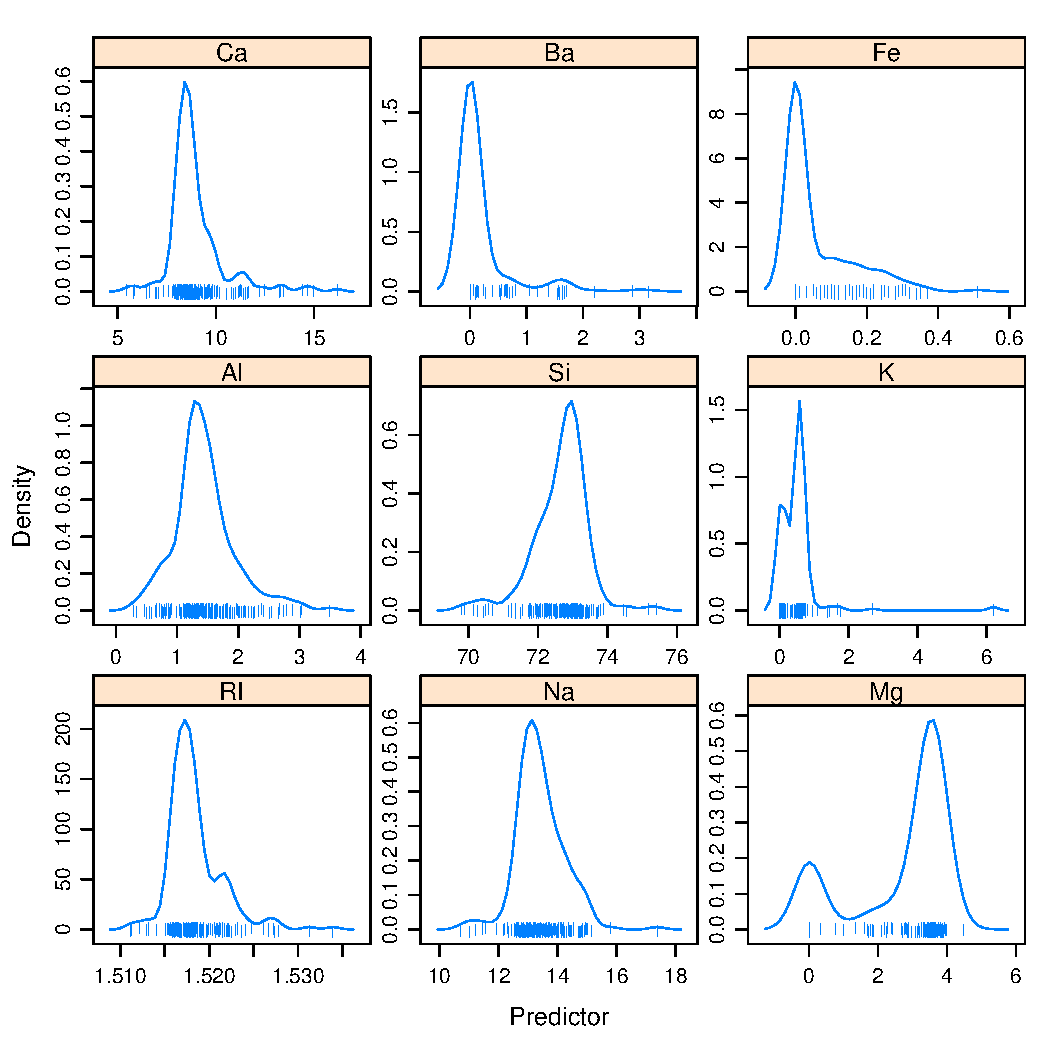
\includegraphics[width=.9\linewidth]{./glassDensityPlots.pdf}
\end{frame}
\begin{frame}
\frametitle{Glass dataset: single classification tree}
\label{sec-1-1-5}


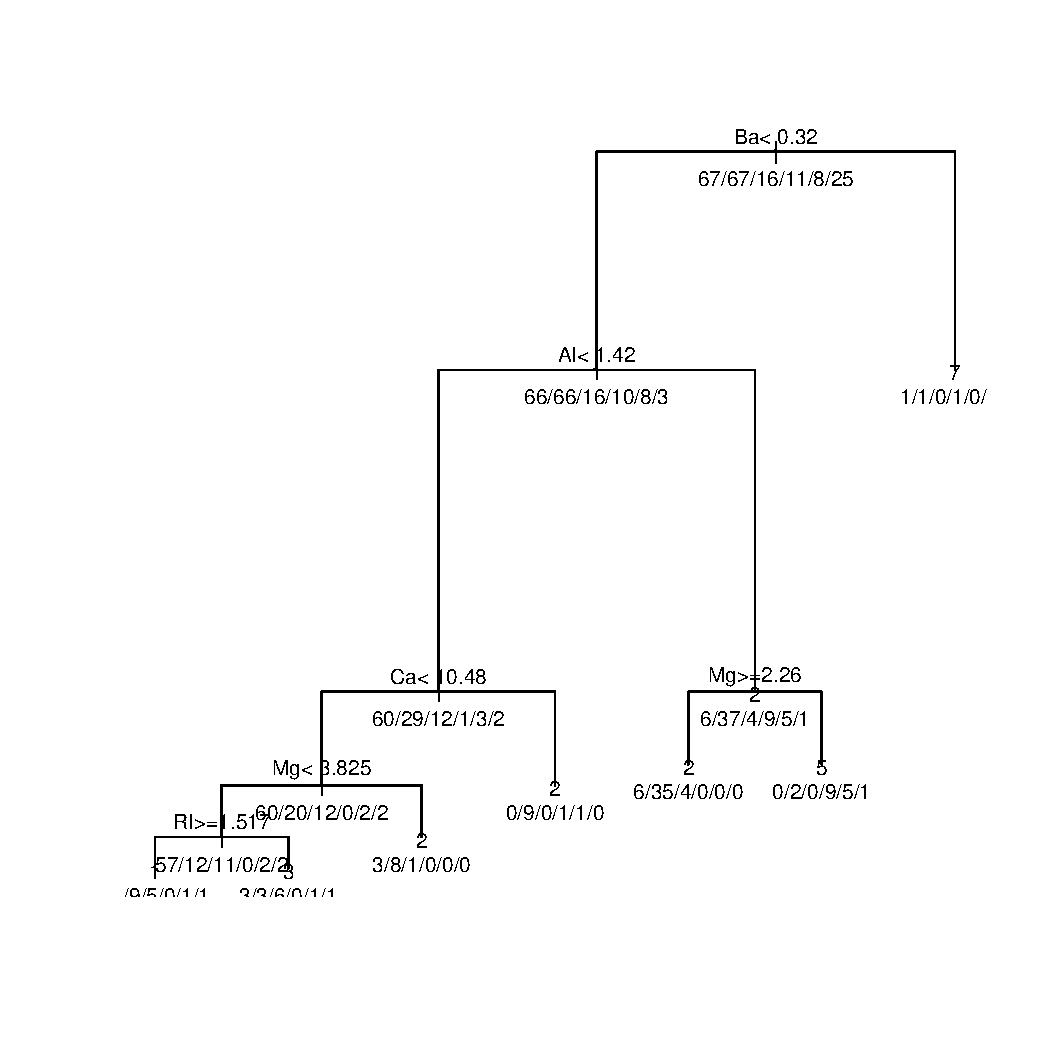
\includegraphics[width=.9\linewidth]{./onetree.pdf}
\end{frame}
\begin{frame}
\frametitle{Different Learning Sets Create Different Trees}
\label{sec-1-1-6}


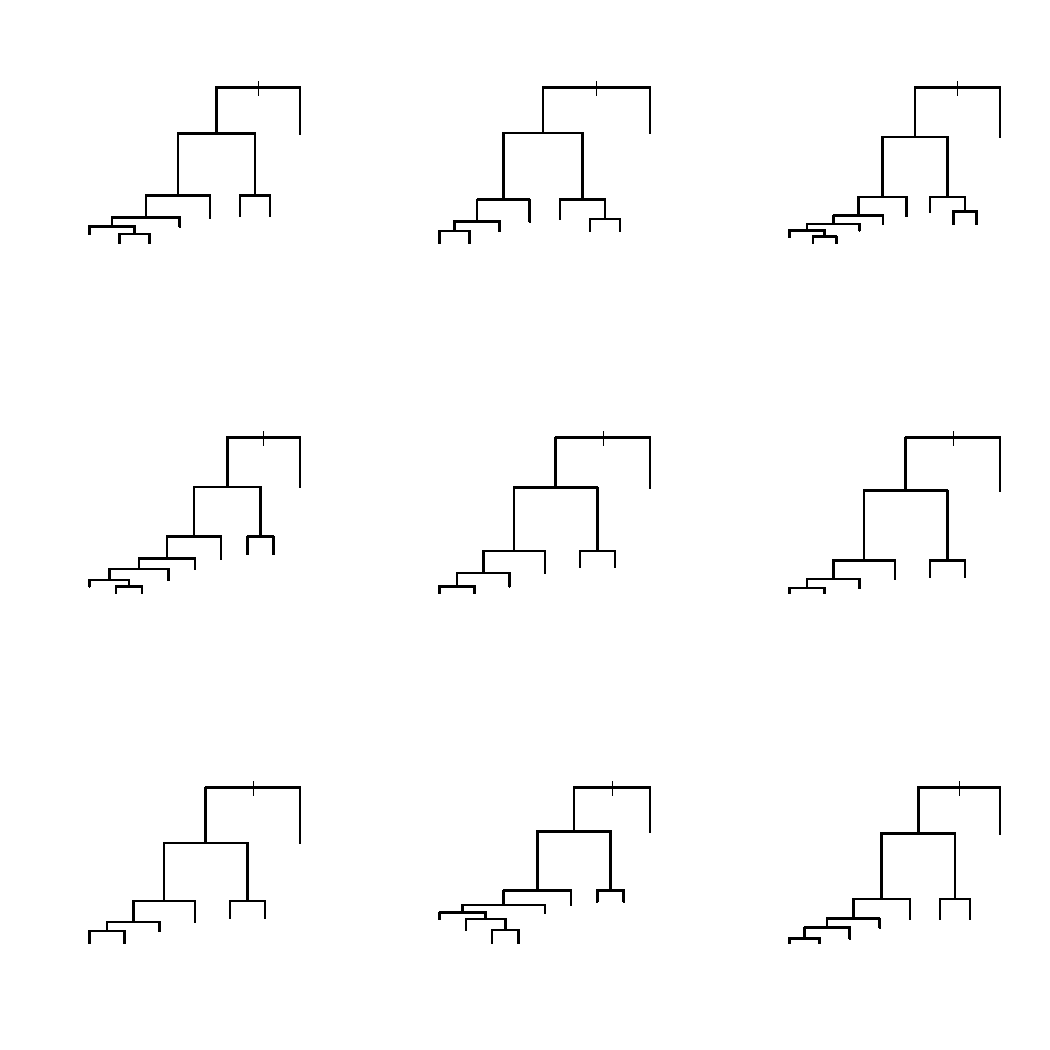
\includegraphics[width=.9\linewidth]{./diffTrees.pdf}
\end{frame}
\subsection{Bagging basics}
\label{sec-1-2}
\begin{frame}
\frametitle{Bagging definition}
\label{sec-1-2-1}
\begin{itemize}

\item ``bagging'' bootstrap aggregation\\
\label{sec-1-2-1-1}%
uses resampling as a smoothing device
\begin{itemize}
\item prediction and nonparametric classification problems
\item useful when basic algorithm is unstable after small data perturbations
\end{itemize}


\item Notation\\
\label{sec-1-2-1-2}%
\begin{itemize}
\item data $d = \{(x_j,y_j),j=1,\ldots,n\}$
\item response $y$ numerical or class
\item predictor $x\equiv (x^{(1)},\ldots,x^{(p)})$
\item predictor formula $m_0(x|d_n)$
\end{itemize}

\end{itemize} % ends low level
\end{frame}
\begin{frame}
\frametitle{Bagging overview}
\label{sec-1-2-2}


\begin{itemize}
\item empirical bagged predictor, acts as asmoother which reduces
  variance.
\item can reduce MSE of predictor by 50\%
\item bagging by voting: pick the class which is choosen most often in R
  resamples
\item ``boosting'' attaches weights to the data according to difficulty clasifying.
\end{itemize}
\end{frame}
\begin{frame}
\frametitle{Bagging schematic}
\label{sec-1-2-3}


\begin{enumerate}
\item Resample the data: $d \rightarrow d^{\star}_1,\ldots,d^{\star}_R$
\item Construct predictors: $m_0(x|d^{\star}_1),\ldots,m_0(x|d^{\star}_R)$
\item Bagged predictor is an average: $$\hat{m}_B(x|d) = \frac{1}{R}
   \sum_{r=1}^{R}m_0(x|d^{\star}_r)$$
\end{enumerate}

Approximates $m_B(x|d) = E^{\star}\{m_0(x|D^{\star})\}$.
\end{frame}
\subsection{Bagging in action}
\label{sec-1-3}
\begin{frame}
\frametitle{Classification scheme stability (Breiman 1994)}
\label{sec-1-3-1}



\begin{center}
\begin{tabular}{ll}
 Stable             &  Unstable                               \\
\hline
 k-nearest neighor  &  Neural nets                            \\
                    &  Classification trees                   \\
                    &  Regression trees                       \\
                    &  Subset selection in linear regression  \\
\hline
\end{tabular}
\end{center}



\begin{itemize}
\item Bagging is useful in unstable cases
\item Typical number of bootstrap replicates is $\sim$ 50
\end{itemize}
\end{frame}
\begin{frame}
\frametitle{Cross-Validation (Petersen et al. 2008)}
\label{sec-1-3-2}


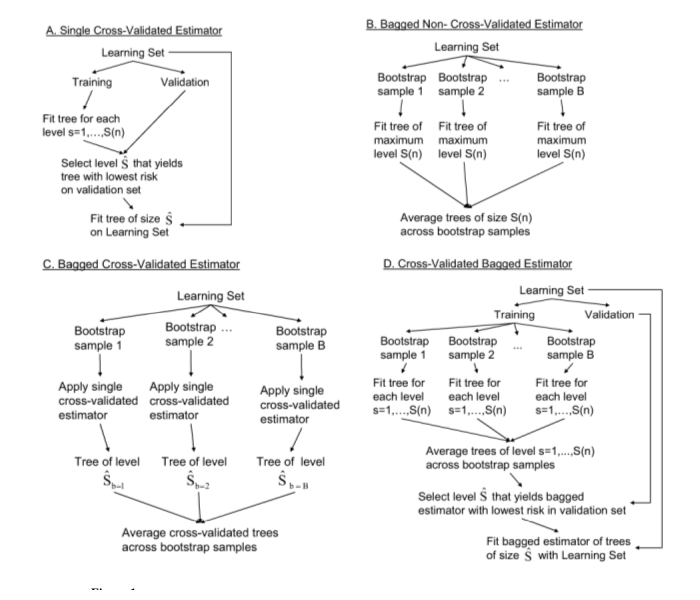
\includegraphics[width=.9\linewidth]{./PetersenFig1.png}
\end{frame}
\begin{frame}
\frametitle{Misclassification rate reduction with bagged classification trees (Breiman 1996)}
\label{sec-1-3-3}

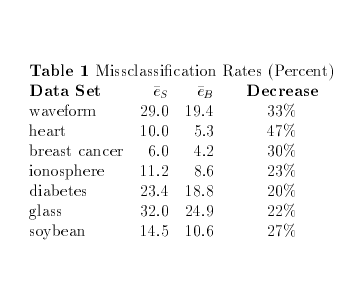
\includegraphics[width=.9\linewidth]{./Btable1.png}
Breiman1996
\end{frame}
\begin{frame}
\frametitle{Screening of predictor variables}
\label{sec-1-3-4}
\begin{itemize}

\item Hard thresholding example
\label{sec-1-3-4-1}%
\begin{itemize}
\item linear regression formula with screening of predictor variables
\end{itemize}
$$m_0(x|d) = \sum_{i=1}^{p} \hat{\beta_i}
I(|\hat{\beta_i}|>c_i)x^{(i)}$$


\item Bagged predictor does ``soft thresholding.''\\
\label{sec-1-3-4-2}%
$$m_B(x|d_n) = \sum_{i=1}^{p} E^{\star}\{\hat{\beta^{\star}_i} I(|\hat{\beta^{\star}_i}|>c_i)\}x^{(i)}$$

\end{itemize} % ends low level
\end{frame}
\begin{frame}
\frametitle{Buhlmann and Yu (2002)}
\label{sec-1-3-5}

\begin{itemize}
\item Bagged indicator example shows how bagging converts a
  hardthresholding desicion to softthresholding (smoothens)
\end{itemize}

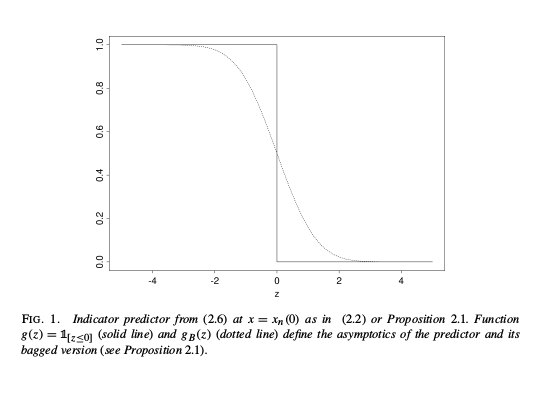
\includegraphics[width=.9\linewidth]{./BuhlmannYuFig1.png}
\end{frame}
\subsection{Conclusions}
\label{sec-1-4}
\begin{frame}
\frametitle{Advantages of Bagging}
\label{sec-1-4-1}

\begin{itemize}
\item Bagging is useful for unstable predictors
\begin{itemize}
\item aggregation reduces variance and makes predictions more stable
\end{itemize}
\item Useful for high-dimensional case
\begin{itemize}
\item also shown to be successful in smaller problems (Buja and
    Stuetzle 2000)
\end{itemize}
\item Out-of-bag: use samples that were not selected by bootstrap to
   measure predictive performance
\end{itemize}
\end{frame}
\begin{frame}
\frametitle{Bagging Pitfalls}
\label{sec-1-4-2}

\begin{itemize}
\item Less interpretable than single model
\item Poor classification predictors can become worse (Breiman 1996)
\item Increase computational complexity/demand
\end{itemize}
 
\end{frame}
\subsection{Questions?}
\label{sec-1-5}

\end{document}
